En general, sabemos que las fluctuaciones cambiarias componen uno de los riesgos más importantes a los que se enfrentan los inversionistas. Por ello es de gran importancia realizar el pronóstico de volatilidad para la toma de decisiones relacionadas con la administración de portafolios. De esta forma, los modelos denominados de heteroscedasticidad condicional autorregresiva nos permiten realizar una buena estimación. 
\\\\
Hsieh (1989) sostiene que en la familia de los modelos ARCH/GARCH no hay uno que se
pueda considerar como el modelo general para pronosticar los diferentes tipos de cambio.
Sin embargo, es conveniente señalar que en particular el uso del modelo GARCH se
justifica porque permite especificaciones más parsimoniosas que el modelo ARCH, sus propiedades son bastante conocidas porque es la especificación más común entre los modelos de la familia ARCH/GARCH y se ajusta muy bien a los datos de variables financieras, principalmente
cuando las observaciones son de alta frecuencia. \footnote{Ortiz-Arango, F., \& Cabrera Llanos, A. (2012). Pronóstico de la volatilidad cambiaria peso-dólar mediante modelos GARCH (pp. 3-5). México.}

 Para un periodo de 20 días, (aproximadamente un més de cotizaciones), hicimos uso de la función \textit{ugarchforecast()} la cual nos permite obtener las bandas de confianza dentro de las cuales se espera que  los rendimientos futuros se encuentren (Figura \ref{pronostico_serie}) y por otro lado, también nos permitió obtener el comportamiento futuro de la varianza de dichos rendimientos. (Figura \ref{pronostico_varianza})
\begin{figure}[!ht]
    \centering
    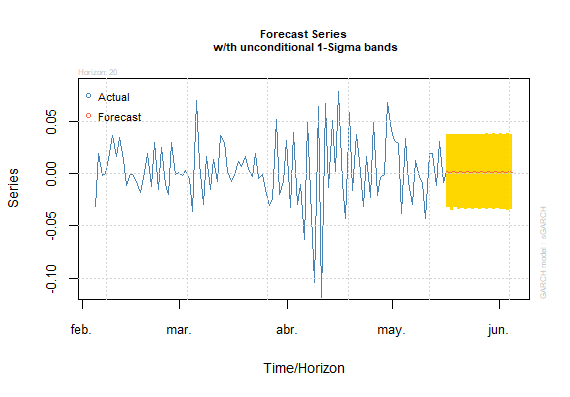
\includegraphics[scale=.8]{Graficos/pronostico_serie_20dias.png}
    \caption{Pronóstico de rendimientos con bandas}
    \label{pronostico_serie}
\end{figure}

\begin{figure}[!ht]
    \centering
    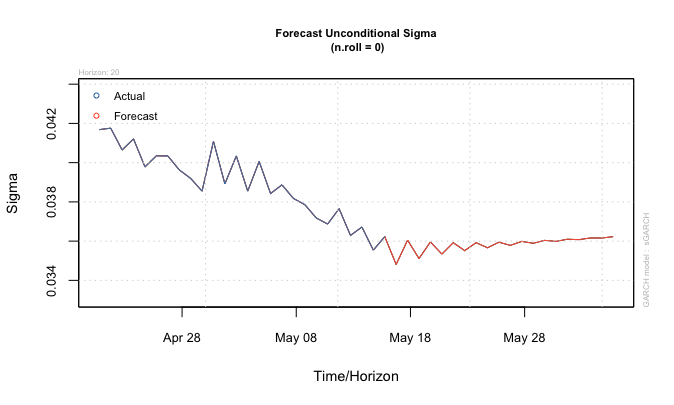
\includegraphics[scale=.5]{Graficos/Pronostico de Varianza.png}
    \caption{Pronóstico de varianza}
    \label{pronostico_varianza}
\end{figure}

\newpage
Recordando que el pronóstico para este tipo de modelos se basa en el valor esperado de las innovaciones y, por lo tanto, en la densidad elegida. Los pronósticos de un paso adelante se basan en el valor de los datos anteriores, mientras que los n pasos adelante (n$>$ 1) se basan en la expectativa incondicional de los modelos. Por esto, las gráficas anteriores muestran datos bajo la volatilidad ``unconditional``. La capacidad de lanzar el pronóstico un paso a la vez se implementa con el argumento \textit{n. Roll}, que controla cuántas veces se debe lanzar el pronóstico n. Adelantado. El argumento predeterminado de \textit{n. Roll = 0} denota que no hay desplazamiento y devuelve el pronóstico n. Anticipado estándar. Fundamentalmente, dado que n. Roll depende de que haya datos disponibles para basar el pronóstico móvil.
\\\\
Como podemos observar de la Figura \ref{pronostico_serie} y la Figura \ref{pronostico_varianza} , aquella que muestra las bandas de confianza de los rendimientos hace evidente que para el siguiente mes se tiene esperado un comportamiento poco volátil, considerando que en periodos anteriores los rendimientos habían fluctuado de manera agresiva. Esto se ve reafirmado por el gráfico de la varianza estimada, pues es claro que tiende a estabilizarse con el tiempo. 

